\Chapter{Related Work}\label{chapter:related}

All events happening within the game world form the plot of the game.
The way the plot is presented to the player depends on the narrative.
In other words the narrative is the plot with added context and presented using a certain storytelling technique.
The reception of the narrative by the player is often less dependent on the plot than it is on the technique used to present it.
In this thesis, the focus is not on the narrative but rather just the formal representation of the plot itself.
The plot consists of all events, characters and their actions in the game, all of which do not need to be available to the player or even exist in any way as separate beings.
Characters and their actions can be parts of the plot in the form of writing or recordings and events can be referenced in the history of the simulated world even though they were never really represented.
The actual form of the plot depends on the type of the game and the narrative it tries to establish.
As noted by Lindley, the plot state of the game world does not need to be available and presented to the player in its entirety, as is the case for example in games such as SIM City \cite{lindley2005story}.
In many games the player experiences a subset of the available plot and thus forms their own customized narrative.

Saussure\cite{gordon2004langue} introduced the distinction between language (fr. \emph{la langue}) and meaning (fr. \emph{la parole}).
This distinction is similar to the difference between plot and narrative and likewise applicable in the context of plot representation alone.
In Saussure's framework, language refers to the overall system of rules, conventions, and structures that govern a particular language, while meaning refers to the individual utterances or expressions produced by speakers of that language.
This distinction emphasizes the idea that language is a system that is shared and agreed upon by a community of speakers, and that meaning is not fixed but rather is created through the interaction between the language system and the speaker's intentions and context.
When representing the plot state of a game world, it is important to consider the language used to describe that world and the range of expressions that are possible within that language.

The two most commonly used formalisms for representation of situations and their development in time are situation calculus and event calculus.
The situation calculus is a logical language for representing changes\cite{lin2008situation}.
According to Levesque, in situation calculus "the foundational axioms for situations provide a purely qualitative notion of time whose only temporal concept is sequential action occurrence: an action occurs before or after another within"\cite{levesque1998foundations}.
The event calculus is a formalism for reasoning about action and change \cite{mueller2008event}.
Similarly to the situation calculus, the event calculus uses the concept of actions (called "events") and fluents.
The main difference is that events can be external and happen at specific time points which makes it essential for modelling plot state where a plot event can happen in isolation.
Event calculus was introduced first in 1986 by Kowalski and Sergot \cite{kowalski1986logic}.
It was then simplified in 1992 \cite{kakas1992abductive}.
In general, the ontology of event calculus includes the definitions of fluents and actions.
Fluents describe the state of the plot and can change in time as a result of an action.
This approach can be used to model and reason about flow of events but no example of its application in game development has been found in literature.
One of the major limitations of event calculus is its rigidity and inability to produce generative content as it is only used to describe already existing sequences of events.

A plot in a game can be implemented using a script by the game designer or it can emerge naturally during gameplayer based on the interactions between individual elements in game.
The former approach is usually implemented in role playing games as game designers and writers collaborate to bring to life the creative vision for a given imaginary world.
On the other hand, games such as Dwarf Fortress use simulation of individual interactions between game elements to formulate a plot \cite{adams2015simulation}.
This in turn leads to a phenomenon called emergent behavior where an interaction of simple elements produces a complex behaviour \cite{adams2019emergent}.
Emergence in game design is not a new concept and is used frequently in the game development industry \cite{sweetser2008emergence}.
While it can increase immersiveness and replayability, it also increases the overall complexity of both gameplay and development.

Games that lean heavily towards utilization of emergent behaviours usually depend on multi-agent simulation where each agent represents either a non-playable character (NPC) or the player themselves.
Agents that are controlled by the game and not the player have builtin interaction rules and behaviours that allow them to act in a way that is expected and realistic in a given scenario.
Agent-based simulation (ABS) has been used for a long time already and can be applied to any given game genre including some well known zero-player games such as Game of Life \cite{chan2010simulation}.
In these simulations agents have their own mememory and ability to process information, eventaully integrating it into knowledge that is used for choosing the response to any situation that can happen within the rules of the game.

% What is data, information, knowledge?

To understand how agents work with information, the concept of information and its relationship to knowledge needs to be explained.
The earliest work discussing information and similar concepts comes from Shannon in 1948\cite{shannon1948mathematical}.
The author however never defines the term itself and simply proposes models for quantitative analysis.
Approach described back then was more related to data than it was to information.
The distinction was made clear by Langefors in 1973\cite{langefors1973theoretical}.
Langefors proposed an approach putting the users of information first and proposed the following equation to describe the interaction of time, data, knowledge and information:
$$
    I = i(D, S,t)
$$
where:
\begin{variables}
    $I$ & information \\
    $i$ & interpretation process \\
    $D$ & data \\
    $S$ & knowledge \\
    $t$ & time
\end{variables}
In 1989, Ackoff\cite{ackoff1989data} defined the hierarchy of the human mind as consisting of wisdom at the very top and descending into understanding, knowledge, information and further into data.
The more popularized variant of this hierarchy being DIKW (data, information, knowledge, wisdom), became widespread in literature regarding knowledge management\cite{skyrme2007knowledge}.
There have been many attempts to define the distinction between these terms as well as the terms themselves.
One notable example was done by Grabowski and Zając in 2009\cite{mariusz2009dane}.
\begin{figure}[H]
    \centering
    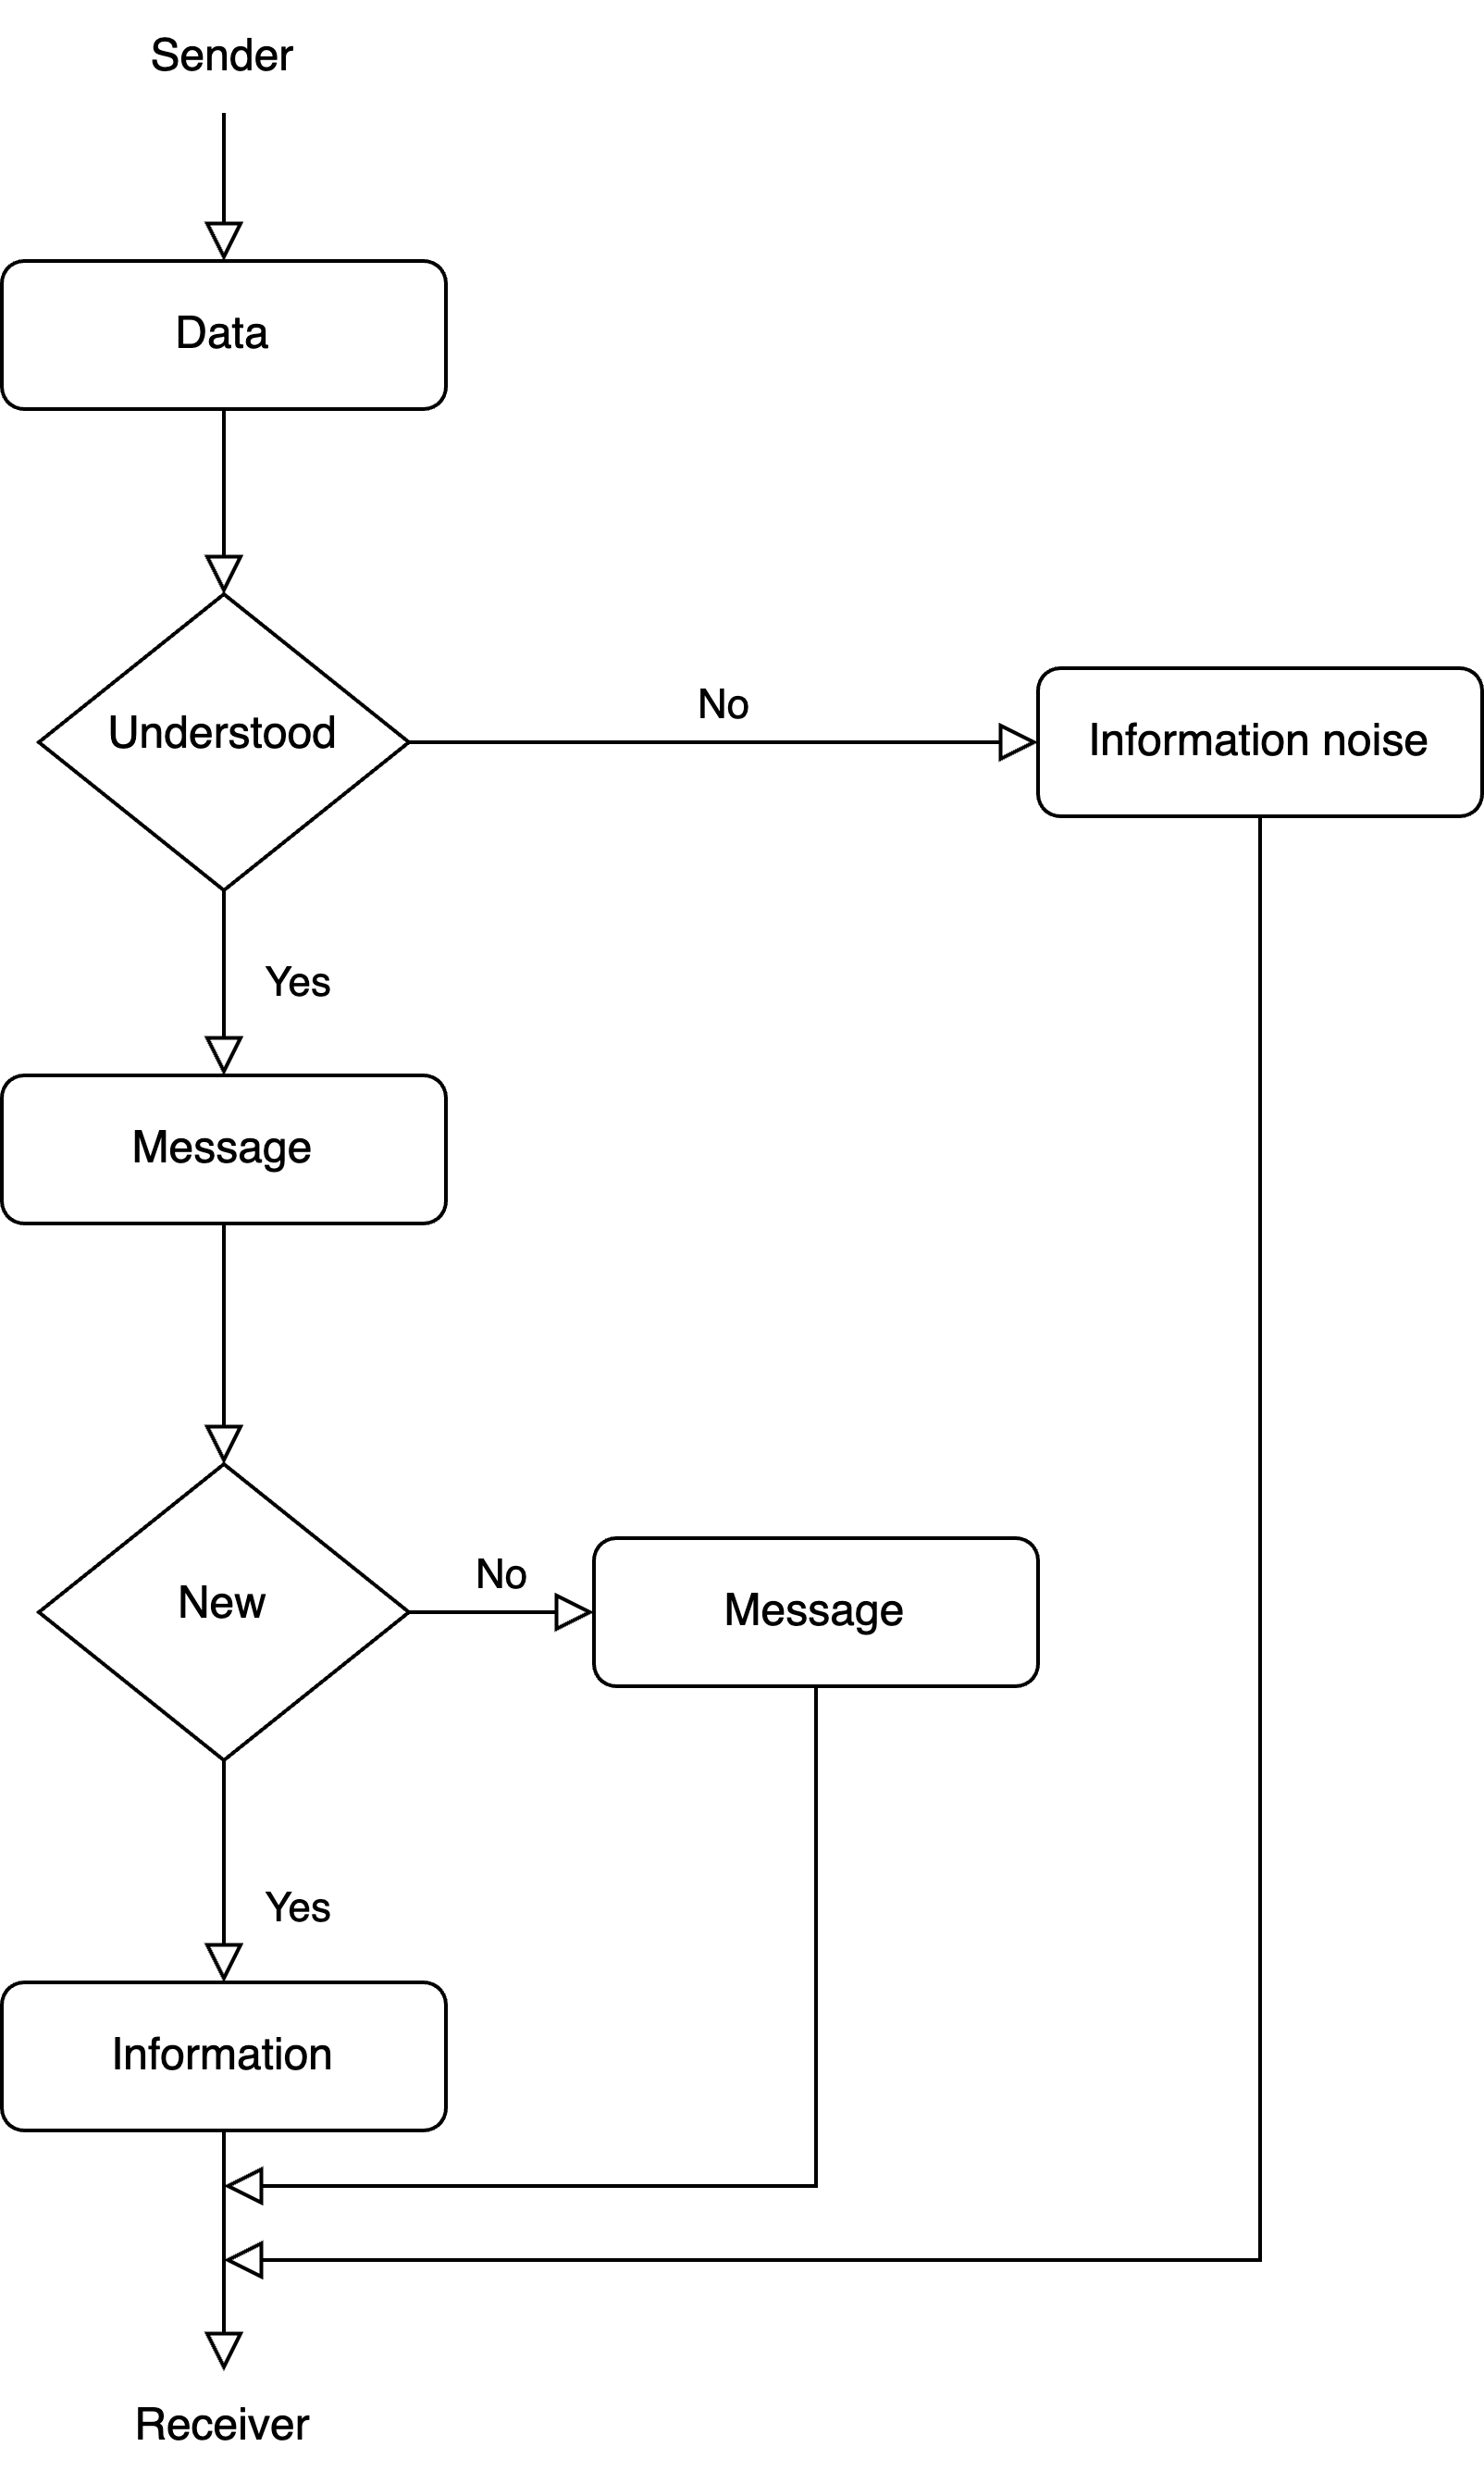
\includegraphics[width=0.5\textwidth]{images/od_nadawcy_do_odbiorcy.png}
    \caption{Information flow\cite{mariusz2009dane}}\label{fig:od_nadawcy_do_odbiorcy}
\end{figure}
The authors stress the hardship of definition of such primal terms and highlight the two major science disciplines that are related to them (information theory and knowledge management).
Both disciplines use the pyramid of knowledge (or information respectively).
According to Liew\cite{liew2013dikiw} trying to accurately define data, information and knowledge will result in circular definition.
To solve that problem he proposes a DIKIW model where "I" stands for "Intelligence".
Irrespective of chosen framework, everyone agrees that information and knowledge are related but represent different levels of abstraction.
While data is raw and unprocessed before it can become information, similarly information needs to be retained and assimilated to become knowledge.
The scope of this thesis covers only information understood as statements of fact and knowledge defined as retained and processed information.

A population of people can be said to possess knowledge similarly to a single individual.
Often a crowd has greater knowledge than any individual.
Surowiecki said "under the right circumstances, groups are remarkably intelligent, and are often smarter than the smartest people among them"\cite{surowiecki2005wisdom}.
To understand how knowledge is gained within a population one should analyze the way information itself is propagated.
In fact, people have already noticed that certain facts, stories or news share similarities with viral infections in how they spread across the whole population and eventually die out.
One such example is the work done by Liu et al.\cite{liu2016} where the authors describe how information spread can be explained using epidemiological models.
Truly, the simplest of such models called SIR\cite{weiss2013sir} can be used to describe in simple terms how a population can be partitioned into groups of \emph{Susceptible} (people who haven't encountered the viral information yet), \emph{Infected} (those who know the news and are willing to share it) and \emph{Removed} (everyone who either lost interest or simply never exhibited it).
There are however differences between infectious diseases and information.
For this reason variations of the SIR model became born.
Zhao et al.\cite{zhao2012sihr} have developed the SIHR model where H stands for \emph{Hibernators}.
The authors stress the importance of forgetting and remembering in trying to model the spread of information.
Another variation worth noting is the SCIR model consisting of \emph{Susceptible}, \emph{Contacted}, \emph{Infected} and \emph{Refractory}\cite{xiong2012scir}.
Both models use complex systems in order to simulate information propagation.
Other attempts at modelling information propagation are networks\cite{rodriguez2013} and cellular automata\cite{silva2020}.
Most literature dealing with the topic refers to social media, blogs and internet as the main medium of information exchange.
Relatively few works analyze the mechanisms behind word-of-mouth communication.
In 2003 at the "Symposium on Applications and the Internet", Takeuchi, S. and Kamahara, J. and Shimojo, S. and Miyahara, H. have presented their work titled "Human-network-based filtering: the information propagation model based on word-of-mouth communication" which deals with simulating how certain information is spread based on the filters of interest\cite{takeuchi1183031}.
Most authors treat knowledge of information as a binary value.
In reality the level of knowledge is often more complicated.
Silva et al.\cite{silva2020} propose the application of cellular automata to model information expressed as a linear value.

When trying to model how information propagates in a given system, it is often helpful to try and list its characteristics.
Grabowski and Zając followed the steps of Langefors and others while describing the following set of information characteristics:
\begin{itemize}
    \item Completedness - information must inlude context necessary for its interpretation
    \item Versatility - information should be interpretable from multiple viewpoints
    \item Accuracy - it should not be too vague nor too specific
    \item Financially viable - it should be useful in business context
\end{itemize}
These show clearly how most work done previously in this domain of knowledge related to the business context.

It is apparent that information as utilized in agent-based simulation games is different than the concept used in information theory and derived works.
Social agents that interact with each other and simulate conversations, emotional state and organic behaviour have been analyzed since well before the development of artificial intelligence and language models.
A notable example is the work done by Grey et al. in 2011 titled "Procedural quests: A focus for agent interaction in role-playing-games"\cite{grey2011procedural}.
The author describes the problems with contemporary games and their shallow plot propagation mechanisms and proposes their approach of modelling plot and its propagation using a social multi-agent system.
Very recently many articles have been published that utilize the developments in the area of language models and natural language processing in general.
Park et al.\cite{park2023generative} have used the GPT-4 model\cite{openai2023gpt4} to simulate a small village populated by characters each with individual personality and motivations.
The characters held conversations, organized meetings and socialized in their free time.

In order to simulate with any degree of precision the evolution of plot state in a game, one must take into account the inherent time structures used in said game.
These temporal structures are inherently tied to the game rules which limit the scope of a valid game space and thus influence the rate and shape of plot evolution.
Lindley describes moves in games as "an abstraction over player action, mapping action to a specific significance within the rule set and independent of local, personal and idiosyncratic variations in performance" \cite{lindley2005story}.
They illustrate this by an example of the game of chess where a player may make a move when it is their turn and the space of available moves is limited to a very small subset of all valid chess moves.
There are two major types of time structures in games:

\begin{itemize}
    \item discrete - turns, moves, matches, rounds, etc
    \item continuous - simulation of the passage of time, can use simulation steps with fixed unit of time in-between or dynamic
\end{itemize}

The first kind of temporal structures is easy to reason about and model because it is computationally less intensive than simulating the world and in turn the evolution of plot state as often as possible (or at the very least very frequently to keep the illusion of continuity).
The second kind is much often encountered in contemporary video games which often include physics, weather and daytime simulation as well.
For the sake of simulating propagation of plot events, one can choose to artifically divide the continuous time structure of the game into discrete simulation steps with fixed timestep or rely on the event based model.
An example of such event would be two characters meeting which would trigger the simulation of plot state evolution between them.
The second approach is hard to measure and model without introducing a framework of simulation capable of simulating arbitrary routines of actors within the game world.
For this reason and because the first approach can be adapted to the second scenario as well, the approach described in the subsequent sections deals only with discrete time structures.

In conclusion it can be seen that the use of agent-based simulation in game development is a growing field of research.
Artificial intelligence and its derivatives drive the current state of the art in this area.
Alternative approaches such as proposed back in 2011 by Grey\cite{grey2011procedural} should be explored to compete with the indeterministic nature of language models or perhaps to become the benchmarks against them.

In multi-agent simulation agents within the system are trated as independent entities interacting with each other.
Both the player and any non-playable characters can be called agents.
Each agent is independent from the rest and is able to act based on the subset of the plot available to them.
The actual implementation of each agent's behaviour can be as simple as a hardcoded line of dialogue and as complex as a set of rules enabling emergent behaviour.
General plot of the game as experienced by the player is the sum of interactions and sub-plots of the individual agents in the game.
Grey et al.\cite{grey2011procedural} proposed a solution using agent-based simulation to create procedural quests.
This work focuses on extension of the original approach using a SOAR cognitive architecture\cite{rosenbloom1993soar}.
In order to produce natural interactions between agents, the implementation must not be reliant on user-defined scripts and scenarios and instead should allow expression of the agents' behaviour using a set of independent rules.

According to Langley et al.\cite{langley2009cognitive} a cognitive architecture specifies the underlying infrastructure for an intelligent system.
The authors describe the distinction between the agent's architecture and its memory and beliefs that can change over time, even proposing an analogy to a building with furniture in it, indicating that while the architecture of the building is constant, the elements within are not.
Among the architectures described by the authors are the following examples:

\begin{description}
    \item[ACT] Modular architecture focused on modelling human behaviour. Notable feature of this architecture is that each production rule is associated with a utility function that calculates the potential benefit from execution of the action.
    \item[SOAR] Architecture consisting of production rules and operators that influence the external or internal state of the agent.
    \item[ICARUS] ICARUS splits the memory into concepts, percepts and skills. The concepts and percepts describe the situation while skills allow for choosing an action to take. Skills represent goal concepts they aim to achieve. All memories are stored in a hierarchical way.
    \item[PRODIGY] This architecture defines the concept of domain rules that encode the conditions under which actions can be executed as well as control rules that define which actions are to be selected or rejected.
\end{description}

Another notable example in the space of cognitive architectures is belief-desire-intention (BDI) described by Georgeff in 1992\cite{georgeff1992abstract}.
In this architecture the agents hold certain beliefs about its state, has desire to act in a certain way and possesses intention that guarantees that it does not act randomly.

All cognitive architectures can be used to solve similar problems, albeit each with a different approach.
In this thesis the SOAR (State, Operator, And Representation) architecture was chosen \cite{laird2019soar}.
It allows the agents to have a set of rules that determine their behaviour as well as represent the state of the world as perceived by the agent in its working memory.
The simplicity and straightforwardness of SOAR is one of the main reasons for choosing this particular cognitive architecture.
Additionally, architectures that rely on utility functions that calculate the applicability of a production rule were excluded due to the fact that definition of utility for many aspects of simulation of a virtual character in game is adding extra complexity.
Another beneficial property of SOAR is the ability to express the production rules as independent and non-hierarchical.
In some games decision trees are enough to express the range of interactions with an agent\cite{sweetser2002current}.
The main limitation of this approach is that decision trees are hierarchical and no choice can be made in isolation as well as the fact that they are usually deterministic and thus predictable.
The latter limitation is avoidable as probabilistic decision trees can be used \cite{saks1986probabilistic}, however the former limitation is a characteristic of all trees and relational graph structures.

SOAR is a cognitive architecture that is designed to simulate human thinking and problem-solving processes.
At its core, SOAR is a symbolic, production-based system that uses rules to guide behavior.
All production rules in this architecture are independent and concerned with a single specific behaviour or inference that the agent can perform.
The memory can store hierarchical information but the rules that govern the agent's behaviour are not hierarchical themselves.

This architecture consists of two major components:

\begin{itemize}
    \item Procedural memory (production memory) - set of production rules that take working memory elements and propose operators (behaviours) or modify the state of working memory (inferences)
    \item Working memory - fact based knowledge represented by a symbolic graph structure describing the current state of the world
\end{itemize}

Many implementations of this architecture additionally include the concept of long-term memory structure that accumulates knowledge during the whole lifetime of the agent.
In general, implementation of the SOAR architecture can be called a production system.
Unlike many traditional production systems however, all rules that match against the current state of the world will fire (execute actions) in parallel.
This means that the list of rules is not ordered and conflicting operators may be proposed.
In such cases the usual strategy is to create a substate of the working memory with a new goal of conflict resolution.

The SOAR architecture has been successfuly utilized in creation of video game AI agents.
Examples include the application of this architecture to create an autonomous agent designed for playing Quake\cite{laird2001knows}, StarCraft\cite{turner2013soar-sc} and Descent 3\cite{van1999developing}.
Michael van Lent and John Laird in their work "Developing an Artificial Intelligence Engine"\cite{van1999developing} describe a decision cycle in an inference machine:
Based on this fact, the SOAR architecture was chosen as the basis for implementation of the multi-agent system.